% Based on the fei-template.tex
% https://github.com/douglasrizzo/Classe-Latex-FEI/blob/master/fei.cls

%%%% -- PDF/A
%\begin{filecontents*}{\jobname.xmpdata}
\begin{filecontents*}{mestrado.xmpdata}
    \Title {Comparação de Modelos de Embeddings para Recuperação de Código-Fonte a partir de Linguagem Natural}
    \Author {Adalberto Nassu Pompolo}
    %\Copyright {Copyright \copyright\ 2021 "Douglas De Rizzo Meneghetti"}
    \Keywords {busca de código-fonte\sep recuperação de código-fonte\sep linguagem natural\sep transformers\sep embedding}
    \Language {pt-BR}
\end{filecontents*}

\documentclass[font=arial, algo-as-figure, acronym,final, twoside]{fei}
%\documentclass[font=arial, algo-as-figure, acronym, twoside, deposito]{fei}

%\pagestyle{headings}

\usepackage{afterpage}
\usepackage{amsfonts}
\usepackage{amsmath}
\usepackage{array}
\usepackage{colortbl}
\usepackage{comment}
\usepackage{csquotes}
\usepackage{easytable}
\usepackage{here}
\usepackage{indentfirst}
\usepackage[utf8]{inputenc}
\usepackage{lipsum}
\usepackage{listings}
\usepackage{longtable}
\usepackage{multicol}
\usepackage{multirow}
\usepackage{microtype}
\usepackage{pdflscape}
\usepackage{pgfgantt}
\usepackage{setspace}
\usepackage{stmaryrd}
\usepackage{tabularx}
\usepackage{tikz}
\usepackage{url}
\usepackage{graphicx}
\usepackage{caption}


% Add andle brackets to comply with FEI (https://fei.edu.br/biblioteca/manual/manual.pdf)
\DeclareFieldFormat{url}{\bibstring{urlfrom}\addcolon\space<\url{#1}>}

%%%% -- Configuracoes Iniciais
%%%%%%%%%%%%%%%%%%%%%%%%%%%%%%%%%%%%%%%%%%%%%%%%%%%%%%%%%%%%%%%%%%%%%%%%%%%%%%%%%%%%%%%%%%%%%%%%%%%%%%%%%

\author{Adalberto Nassu Pompolo}
%\cidade{Cidade}
%\instituicao{Instituição de Ensino}
\title{Comparação de Modelos de Embeddings para Recuperação de Código-Fonte a partir de Linguagem Natural}
%\subtitulo{subtítulo}

%%%%%%%%%%%%%%%%%%%%%%%%%%%%%%%%%%%%%%%%%%%%%%%%%%%%%%%%%%%%%%%%%%%%%%%%%%%%%%%%%%%%%%%%%%%%%%%%%%%%%%%%%
%%%% -- Entradas Listas de Abreviaturas e Simbolos
%%%%%%%%%%%%%%%%%%%%%%%%%%%%%%%%%%%%%%%%%%%%%%%%%%%%%%%%%%%%%%%%%%%%%%%%%%%%%%%%%%%%%%%%%%%%%%%%%%%%%%%%%
%% -- Commands
\newcommand{\argmax}{\mathop{\mathrm{argmax}}\limits}

% Possibilita quebra de linha em tabela
\newcommand{\specialcell}[2][c]{%
  \begin{tabular}[#1]{@{}c@{}}#2\end{tabular}}

\newacronym[longplural=\textit{Reciprocal Ranks}]{rr}{RR}{\textit{Reciprocal Rank}}
\newacronym[longplural={Campos aleatórios de Markov}]{cam}{CAM}{Campo aleatório de Markov}
\newacronym[longplural=\textit{application programming interfaces}]{api}{API}{\textit{application programming interface}}
\newacronym{fei}{FEI}{Centro Universitário FEI}
\newacronym{pln}{PLN}{Processamento de Linguagem Natural}
\newacronym{bert}{BERT}{\textit{Bidirectional Encoder Representations from Transformers}}
\newacronym{roberta}{RoBERTa}{RoBERTa}
\newacronym{elmo}{ELMo}{\textit{Embeddings from Language Model}}
\newacronym{svm}{SVM}{Máquina de Vetores de Suporte}
\newacronym{nlp}{NLP}{\textit{Natural Language Processing}}
\newacronym{cnn}{CNN}{Rede Neural Convolucional}
\newacronym{ffn}{FFN}{Rede Neural \textit{Feed-Forward}}
\newacronym{dnn}{DNN}{Rede Neural Profunda}
\newacronym{rnn}{RNN}{Rede Neural Recorrente}
\newacronym{bi-gru}{BI-GRU}{Unidade Recorrente Fechada Bidirecional}
\newacronym{gru}{GRU}{Unidade Recorrente Fechada}
\newacronym{mrr}{MRR}{\textit{Mean Reciprocal Rank}}
\newacronym{nbow}{NBOW}{modelo neural de \textit{bag-of-words}}
\newacronym{ndcg}{NDCG}{\textit{Normalized Discounted Cumulative Gain}}
\newacronym{bleu}{BLEU}{\textit{BiLingual Evaluation Understudy}}
\newacronym{ast}{AST}{\textit{abstract syntax tree}}
\newacronym{ncs}{NCS}{\textit{Neural Code Search}}
\newacronym{unif}{UNIF}{\textit{Embedding Unification}}
\newacronym{degraphcs}{DeGraphCS}{\textit{deep graph for code search}}
\newacronym{cdcs}{CDCS}{\textit{Cross-Domain Deep Code Search}}
\newacronym{mman}{MMAN}{\textit{Multi-Modal Attention Network}}
\newacronym{ggnn}{GGNN}{\textit{Gated Graph Neural Network}}
\newacronym{dgms}{DGMS}{\textit{deep graph matching and searching}}
\newacronym{deepcs}{DeepCS}{\textit{Deep Code Search}}
\newacronym{cradle}{CRaDLe}{\textit{Code Retrieval based on statement-level semantic Dependency Learning}}
\newacronym{gnn}{GNN}{\textit{Graph Neural Networks}}
\newacronym{cqil}{CQIL}{\textit{CodeQuery Interaction Learner}}
\newacronym{quecos}{QueCos}{\textit{Query-enriched Code search model}}
\newacronym{coshc}{CoSHC}{\textit{Accelerating Semantic Code Search with Deep Hashing and Code Classification}}
\newacronym{lstm}{LSTM}{\textit{Long short-term memory}}
\newacronym{bilstm}{Bi-LSTM}{\textit{Bidirectional Long short-term memory}}
\newacronym{csrs}{CSRS}{\textit{Code Search with Relevance Matching and Semantic Matching}}
\newacronym{carlcs-cnn}{CARLCS-CNN}{\textit{Co-Attentive Representation Learning Code Search-CNN}}
\newacronym{tbcnn}{TBCNN}{\textit{Tree-based CNN}}
\newacronym{co3}{CO3}{CO3}
\newacronym{coacor}{CoaCor}{\textit{Code annotation for Code retrieval}}
\newacronym{codebert}{CodeBERT}{CodeBERT}
\newacronym{graphcodebert}{GraphCodeBERT}{GraphCodeBERT}
\newacronym{gpt}{GPT}{\textit{Generative Pretrained Transformer}}
\newacronym{gpt2}{GPT2}{\textit{Generative Pretrained Transformer 2}}
\newacronym{tabcs}{TabCS}{\textit{Twostage Attention-Based model for Code Search}}
\newacronym{adacs}{AdaCS}{\textit{Adaptive Deep Code Search}}
\newacronym{birnn}{BiRNN}{\textit{Bidirectional Recurrent Neural Network}}
\newacronym{ir}{IR}{Recuperação de informação}
\newacronym{dl}{DL}{aprendizagem profunda}
\newacronym{resnet}{ResNet}{Rede Neural Residual}
\newacronym{relu}{ReLU}{\textit{Rectified Linear Unit}}
\newacronym{mlp}{MLP}{\textit{Multilayer perceptron}}
\newacronym{bow}{BoW}{\textit{Bag-of-Words}}
\newacronym{bpe}{BPE}{\textit{Byte-Pair Encoding}}
\newacronym{tanh}{Tanh}{\textit{Hyperbolic tangent}}
\newacronym{sql}{SQL}{\textit{Structured Query Language}}


%% -- Listing Configs
% Listing confgis
\lstdefinestyle{xml}{
    language=xml,
    tabsize=2,
    %frame=lines,
    frame=shadowbox,
    rulesepcolor=\color{gray},
    xleftmargin=20pt,
    framexleftmargin=15pt,
    keywordstyle=\color{blue},
    commentstyle=\color{OliveGreen},
    stringstyle=\color{red},
    numbers=left,
    numberstyle=\tiny,
    numbersep=5pt,
    breaklines=true,
    showstringspaces=false,
    basicstyle=\footnotesize\ttfamily,
    emph={type,name,maxOccurs,minOccurs,base,value},
    emphstyle={\color{magenta}}
}

%% - Draws
% Source https://tex.stackexchange.com/a/7045
\newcommand*{\circled}[1]{
    \tikz[baseline=(char.base)]{
        \node[shape=circle,draw,inner sep=2pt] (char) {#1};
    }
}


%%%%%%%%%%%%%%%%%%%%%%%%%%%%%%%%%%%%%%%%%%%%%%%%%%%%%%%%%%%%%%%%%%%%%%%%%%%%%%%%%%%%%%%%%%%%%%%%%%%%%%%

\addbibresource{resources/bibliography/article.bib}

\makeindex

\makeglossaries

\begin{document}

\maketitle
\begin{folhaderosto}
Dissertação de Mestrado, apresentada ao Centro Universitário da FEI para obtenção do título de Mestre em Engenharia Elétrica. Orientado pelo Prof. Dr. Guilherme Wachs.
\end{folhaderosto}
%\begin{folhaderosto}
Dissertação de mestrado, apresentada ao Centro Universitário da FEI para obtenção do título de Mestre em Engenharia Elétrica. Orientado pelo Prof. Dr. Guilherme Alberto Wachs Lopes.
\end{folhaderosto}

\fichacatalografica
\folhadeaprovacao

%\dedicatoria{À minha família, pelo apoio incondicional.}

%\begin{agradecimentos}
%
%\end{agradecimentos}

%\begin{epigrafe}
%	\epig{blabla} {blablab}
%\end{epigrafe}
\begin{resumo}

Ferramentas de busca de código-fonte a partir de linguagem natural são cada vez mais importantes no dia a dia de engenheiros e desenvolvedores de \textit{software}. Atualmente, modelos \textit{transformers} são o estado da arte em diversas tarefas da área de \gls{nlp}, como busca de código-fonte a partir de linguagem natural. Porém, tais modelos requerem muito tempo e recursos computacionais para serem treinados em um determinado domínio (\textit{fine-tuning)}. Por outro lado, redes neurais clássicas como \gls{mlp}, por exemplo, necessitam de menos recursos para seu treinamento, porém não obtém os resultados dos modelos \textit{transformers}. Diante desse contexto, o objetivo do presente trabalho é criar e avaliar um modelo de rede neural para comparação de \textit{embeddings} gerados por redes \textit{transformers} de dois domínios diferentes: linguagem natural e linguagem de programação. Para tanto, serão utilizados seis modelos \textit{transformers}: 3 de linguagem natural e 3 de código-fonte. Além disso, será treinada uma rede neural a fim de encontrar semelhanças entre os \textit{embeddings} gerados por dois domínios diferentes. Com isso, espera-se obter precisão semelhante ao de modelos \textit{transformers} após o \textit{fine-tuning}, sem ser necessário que tais modelos passem por tal processo.
\keywords{busca de código-fonte, recuperação de código-fonte, linguagem natural, transformers, embedding}


\end{resumo}

\begin{abstract}
Code search tools using natural language queries are becoming an essential tool for software engineers. Nowadays, the transformers models are the state-of-art for several natural language processing tasks such as code search using natural language. However, such models requires a lot of computational resources for training in a specific domain (fine-tuning). On the other hand, classical neural networks such as \gls{mlp} takes less computational resources for training in a specific domain, but it does not achieve the transformers models results. In this context, the goal of this paper is to both create and evaluate a neural network model for comparing transformers embeddings from two different domains: natural language and programming language. For this purpose, it will be used six different transformers models: three for natural language and three for programming language. In addition, an neural network will be trained in order to find similarities between the generated embeddings from two different domains. Hence, we hope to achieve similar precision from the transformers models after the fine-tuning, without the need of this process.

\keywords{code search, code retrieval, natural language, transformers, embedding}
\end{abstract}

\glsresetall

%\listoffigures
%\listoftables
%\listofalgorithms
%\printglossaries
\tableofcontents

\chapter{INTRODUÇÃO}
\label{chp:introduction}


Busca de código-fonte é uma tarefa essencial no trabalho de engenheiros e desenvolvedores de \textit{software} \cite{Rahman2018EvaluatingHD}. \textcite{Sadowski2015HowDS} mostrou que, em média, um engenheiro realiza 5 sessões de busca de código-fonte com 12 buscas por sessão, totalizando assim 60 buscas por código-fonte durante um dia de trabalho. \textcite{Xia2017WhatDD} também mostra que trechos de código-fonte estão entre os itens mais buscados pelos engenheiros de \textit{software}.

Porém, um dos problemas conhecidos da área de recuperação de informação é o \textit{term mismatch} ou \textit{vocabulary mismatch} \cite{Furnas1987TheVP} \cite{Carpineto2012ASO}. Em busca de código-fonte, esse problema se dá quando os termos da busca providos pelo usuário não coincidem com os termos utilizados nos trechos de código-fonte correspondentes \cite{Nie2016QueryEB}. Para mitigar o problema de \textit{term mismatch} na busca de código, vem sendo aplicadas técnicas de \gls{nlp} como \textit{query expansion} \cite{Nie2016QueryEB}, modelo booleano \cite{lv2015codehow} e, mais recentemente, modelos \textit{transformers} como o \textit{CodeBERT} \cite{Feng2020CodeBERTAP}.

Atualmente, os modelos \textit{transformers} se tornaram o estado da arte em busca de código-fonte utilizando linguagem natural pelo fato destes serem capazes de adicionar informações semânticas às buscas \cite{Guo2021GraphCodeBERTPC}. Isso significa que tais modelos compreendem, além das informações textuais contidas no trecho de código, informações semânticas sobre o código-fonte como quais tarefas este realiza. Isso reduz o \textit{term mismatch} nas buscas de código-fonte utilizando linguagem natural.

Entretanto, observa-se que o problema de busca de código-fonte lida com dois domínios de linguagem. O primeiro é o da linguagem natural, o qual contempla tanto a descrição do código-fonte quanto os termos de busca fornecidos pelo usuário. Já o segundo domínio refere-se às linguagens de programação, nas quais são escritos os trechos de códigos-fonte que serão buscados. Além disso, modelos \textit{transformers} demandam grande quantidade de recursos computacionais durante seu treinamento em comparação com outros modelos de \textit{machine learning} como \gls{resnet} ou \gls{mlp}.

Diante disso, o objetivo do presente trabalho é comparar modelos de \textit{embeddings} para recuperação de código-fonte a partir de buscas feitas em linguagem natural. Para tanto, será implementado um modelo de comparação de \textit{embeddings}, com parâmetros definidos experimentalmente conforme descrito no capítulo \ref{chp:experiments}, o qual será treinado para comparar a similaridade dos \textit{embeddings} produzidos por modelos \textit{transformers} de linguagem natural e de linguagem de programação.

\section{Objetivo}
O objetivo desse trabalho é criar e avaliar um modelo de rede neural para comparação de \textit{embeddings} gerados por redes \textit{transformers} de dois domínios diferentes: linguagem natural e linguagem de programação. 

\section{Organização do trabalho}
O presente trabalho está organizado da seguinte forma: no capítulo \ref{chp:relatedWorks} é apresentado um retrato do estado da arte das áreas que o presente trabalho abrange, como busca de código e modelos \textit{transformers}. O capítulo \ref{chp:concepts} contém os principais conceitos teóricos abordados no presente trabalho. O capítulo \ref{chp:methodology} apresenta, em detalhes, a metodologia aplicada durante o desenvolvimento do trabalho. No capítulo \ref{chp:experiments} são descritos os experimentos realizados durante o estudo.

\chapter{TRABALHOS RELACIONADOS}
\label{chp:relatedWorks}

O presente capítulo apresenta o estado da arte das duas principais áreas relacionadas ao presente trabalho, Essas áreas, a saber, são: busca de código e processamento de linguagem natural. Os trabalhos apresentados nesses capítulo estão ordenados em ordem cronológica de publicação. Por fim, é apresentada também uma conclusão sobre os trabalhos citados neste capítulo.

\textcite{Sadowski2015HowDS} realizaram um estudo empírico entre desenvolvedores da empresa Google para analisar padrões de busca de código. O estudo foi realizado utilizando duas ferramentas: um questionário com cinco perguntas, que era apresentado ao usuário sempre que este acessava o repositório interno da empresa; e a coleta de registros (logs) gerados por uma ferramenta de busca de código, utilizada pelos usuários do estudo. Os resultados mostraram que programadores realizam, em média, cinco sessões de busca de código, com doze consultas por sessão, por dia de trabalho. Além disso, tais consultas são, geralmente, relacionadas aos seguintes pontos: uso de API; o que o código faz; porque o código está falhando; onde o código está localizado. Como trabalhos futuros, os autores apontam algumas áreas que não foram contempladas pelo estudo em questão, como a qualidade dos resultados da busca e de que forma os resultados da busca são utilizados pelo usuário. 

\textcite{lv2015codehow} notaram que as ferramentas de busca de código existentes tinham dificuldades com consultas em linguagem natural. Por isso, os autores propuseram a \textit{CodeHow}: uma ferramenta de busca de código que utiliza o modelo booleano extendido. Este modelo avalia a similaridade do texto da consulta com a documentação do código, a fim de ranquear os resultados da consulta em questão. Os autores conduziram o estudo com vinte desenvolvedores e estagiários da empresa Microsoft. Ao final, a \emph{CodeHow} obteve $0,794$ utilizando a métrica \textit{Precision@1}, e $0,867$ com a métrica \gls{mrr}. Tais resultados superaram as ferramentas existentes durante o período do estudo, como Ohloh e Apache Lucene. Contudo, os autores levantaram que, como a \textit{CodeHow} não consegue compreender os significados semânticos da consulta e do código, algumas consultas retornaram resultados incorretos. Um exemplo é a consulta "converter uma cor de RGB para HSV", para a qual a \textit{CodeHow} retornava resultados relevantes à consulta "converter uma cor de HSV para RGB". 

\textcite{Gu2018DeepCS} propuseram uma rede neural profunda, chamada \textit{CODEnn}, capaz de relacionar trechos de código com consultas em linguagem natural. Além disso, os autores criaram uma ferramenta de busca de código (\gls{deepcs}), baseada na \textit{CODEnn}, como prova de conceito do estudo em questão. Para relacionar linguagem natural com código, a \textit{CODEnn} aprende as representações vetoriais do par código/descrição, de forma que um trecho de código é relacionado à uma consulta em linguagem natural utilizando o vetor gerado pela consulta. Utilizando este método, os autores obtiveram resultados de busca de código melhores do que ferramentas como Apache \textit{Lucene} e \textit{CodeHow}. Por fim, como trabalhos futuros, os autores pretendem investigar mais aspectos de códigos-fontes, como estruturas de controle, a fim de melhorar a representação de semânticas de alto nível do código-fonte.

\textcite{Chu2019AGA} propôs um sistema para busca de código que combina aprendizagem de máquina baseada em grafos com modelos \emph{transformer}, além de modelos tradicionais de busca como \textit{ElasticSearch} (ferramenta de busca baseada no Apache \textit{Lucene}). O sistema em questão aplicou \emph{embeddings} hiperbólicos e clusterização de grafos aos dados da base \emph{CodeSearchNet} \cite{Husain2019CodeSearchNetCE}, a fim de incorporar a estrutura de grafos presente nos repositórios de código aos modelo de busca testados. Com isso, foram testados os seguintes modelos de busca: \gls{nbow}; \textit{ElasticSearch}; \textit{ElasticSearch} com clusterização de grafos. Utilizando a métrica \gls{ndcg}, comumente utilizada para avaliar mecanismos de busca, obteve-se $0,190$ com o \gls{nbow}, $0,196$ com \textit{ElasticSearch} e $0,208$ com o \textit{ElasticSearch} com clusterização de grafos. Por fim, dentre as melhorias sugeridas pelos autores está a utilização de outros modelos neurais no lugar do \textit{ElasticSearch}, combinados com o modelo de grafos proposto.

\textcite{Cambronero2019WhenDL} analisaram o uso de modelos de aprendizado supervisionado e não supervisionado dentro do contexto de busca de código. Para tanto, os autores criaram uma plataforma comum de testes, e utilizaram \textit{benchmarks} como \gls{mrr}, além de criarem um modelo supervisionado, chamado \gls{unif}, o qual consiste em uma variação de um modelo \gls{ncs} (não supervisionado). Nos testes, os autores obtiveram resultados melhores com modelos supervisionados do que com modelos não supervisionados. Com isso, os autores sugerem o uso modelos de aprendizagem mais simples (como o \gls{unif}) para sistemas de busca de código. Além disso, o estudo mostra que uma base de dados de treinamento que se assemelhe com consultas comuns dos usuário, provê melhorias significativas para todos os modelos supervisionados.

\textcite{Wan2019MultimodalAN} propuseram o modelo \gls{mman} para busca semântica de código. O \gls{mman} utiliza diversos outros modelos, como \gls{lstm}, \textit{Tree-LSTM} e \gls{ggnn}, para representar características do código-fonte. O estudo em questão comparou o \gls{mman} com outros métodos de busca de código (como \textit{CodeHow} e \gls{deepcs}) utilizando as métricas \textit{SuccessRate@k} e \gls{mrr}, além de dados disponíveis no \textit{Github} para criação da base de dados. Com isso, o \gls{mman} obteve os melhores resultados no estudo. Como trabalhos futuros, os autores planejam aplicar o \gls{mman} em outras tarefas de engenharia de software como sumarização de código e detecção de plágio em código-fonte.

\textcite{Yao2019CoaCorCA} propuseram um modelo de aprendizagem por reforço, chamado \gls{coacor}, o qual gera descrições (em linguagem natural) de código-fonte a fim de melhorar modelos de busca de código. Os testes do estudo foram realizados com a base de dados \textit{StaQC} \cite{Yao2018StaQCAS} e utilizando os modelos de busca de código \gls{deepcs} e \textit{CODEnn}, além do \gls{mrr} e \gls{bleu} como métricas para busca de código e geração de descrição, respectivamente. Os resultados mostraram que o \gls{coacor} foi capaz de gerar descrições úteis para trechos de código, e que tais descrições foram capazes de melhorar a performance dos modelos de busca testados.

\textcite{Akbar2019SCORSC} estudaram a combinação de \glspl{cam} com a semântica dos vetores de palavras obtidos pelo algoritmo \textit{word2vec}. Com isso, os autores compararam as sequências de palavras de uma consulta em linguagem natural, e de um código-fonte. Utilizando as métricas \textit{map@k}, \textit{precision@k} e \textit{recall@k}, além das bases de dados \textit{BUGLinks} e \textit{iBUGS}, o estudo em questão obteve melhoras entre $6\%$ e $30\%$ de acurácia na busca de código.

\textcite{Heyman2020NeuralCS} estudaram o impacto que códigos anotados tem em modelos de busca de código. Segundo os autores, um código anotado é um trecho de código com descrições de sua intenção em linguagem natural. Durante o estudo, foram utilizados os modelos de busca de código \gls{ncs} e \gls{unif}, além das bases de dados \textit{CoNaLa}, \textit{StaQC} \cite{Yao2018StaQCAS} e SO-DS, as quais contém códigos em \emph{Python}. Como \emph{benchmark}, foram utilizadas as métricas \textit{recall@3}, \textit{recall@10} e \gls{mrr}. Ao se utilizar código anotado, obteve-se uma melhora de $20.6\%$ no \gls{mrr}, $23,9\%$ no \textit{recall@3} e $26,4\%$ no recall@10, em comparação aos métodos de busca que não utilizam código anotado. Por fim, os autores acreditam que tais melhorias poderão ser notadas mesmo como outras linguagem de programação (como Java, por exemplo), caso seja aplicado o uso de código anotado nos modelos de busca.

\textcite{Yan2020AreTC} observaram dificuldades em se comparar métodos de busca de código, como a falta de uma bases de dados em comum para comparação de dois métodos de busca. Diante disso, os autores realizaram um estudo empírico para comparação de dois tipos de métodos de busca de código a partir de consultas em linguagem natural. Os dois tipos de método em questão são: métodos baseados em \gls{ir}, e baseados em \gls{dl}. Para tanto, os autores criaram uma base de dados com códigos Java, chamada \textit{CosBench}, e utilizaram essa base para comparar quatro métodos de busca \gls{ir} e dois métodos \gls{dl}. Por fim, os resultados mostraram que os métodos baseados em aprendizagem profunda são mais adequados para consultas relacionadas à reutilização de código, enquanto métodos baseados em recuperação de informação são mais adequados para consultas relacionadas à resolução de \emph{bugs} e usos de determinadas \glspl{api}. Como trabalhos futuros, os autores levantam que a intenção da consulta feita pelo programador possa ser inferida automaticamente, de forma a ajudá-lo a encontrar o melhor método de busca para sua consulta.

\textcite{Feng2020CodeBERTAP} propuseram o \textit{CodeBERT}, um modelo bimodal para linguagem de programação e linguagem natural. O \textit{CodeBERT} utiliza uma arquitetura baseada no modelo \gls{bert}. Porém, o \textit{CodeBERT} é capaz de aceitar tanto dados bimodais (par código/linguagem natural) quanto dados unimodais (apenas código). Dados bimodais geralmente são usados para tarefas de busca de código, enquanto dados unimodais para geração de código. Com o \textit{CodeBERT}, os autores conseguiram resultados iguais ou, em alguns casos, melhores do que o estado da arte. As comparações foram feitas utilizando as métricas \gls{mrr} para busca de código e \gls{bleu} para geração de código. Por fim, como trabalhos futuros, os autores apontam a incorporação de \gls{ast} nas fases de pré-treino.

\textcite{Li2020LearningCI} propuseram o \gls{cqil}, um modelo de busca de código que utiliza redes neurais convolucionais para encontrar relações léxicas e semânticas entre a consulta e o trecho de código. A fim de comparação, o estudo utilizou os modelos de busca \gls{deepcs}, \gls{unif}, Apache Lucene e \textit{CodeHow}, bem como as métricas \textit{map@k}, \textit{SuccessRate@k} e \gls{mrr}, além das base de dados \textit{CODEnn} e \textit{CosBench}. Os experimentos realizados mostraram melhora de performance em todas as métricas utilizadas. Além disso, os autores apontam que o \gls{cqil} também possui boa performance com bases de dados pequenas.

\textcite{Ye2020LeveragingCG} utilizaram geração de código para melhor correlacionar linguagem de programação e linguagem natural. Para tanto, o modelo proposto, chamado \gls{co3}, utiliza \textit{dual
learning} e \textit{multi-task learning}. Para os experimentos, os autores utilizaram o banco de dados \textit{StaQC} \cite{Yao2018StaQCAS}, o qual contém trechos de código das linguagens de programação \gls{sql} e \textit{Python}. Utilizando as métricas \gls{mrr} e \gls{ndcg}, os autores obtiveram $0,585$ e $0.682$ (respectivamente) para \gls{sql}, e $0,679$ e  $0,756$ para \textit{Python}. Como trabalhos futuros, os autores planejam explorar as interações entre as perdas de ranking para busca de código.

\textcite{Ling2020AdaptiveDC} propuseram um método de busca de código chamado \gls{adacs}. Este método divide o processo de aprendizagem em duas etapas: aprendizagem de \textit{embeddings} de domínio específico, e aprendizagem de combinações de padrões sintáticos. Isso possibilita ao \gls{adacs} se adaptar à novas palavras, específicas de determinado domínio, mesmo que estas não tenham sido aprendidas durante o treinamento. Para os experimentos, o estudo utilizou códigos escritos em \textit{Java} e disponíveis no \textit{Github} e métodos de busca de código como \textit{CodeHow} e \gls{deepcs}. Utilizando as métricas \gls{mrr} e \textit{hit@k}, o \gls{adacs} obteve resultados melhores em todas as comparações feitas no estudo. Por fim, dentre os possíveis trabalhos futuros, os autores planejam melhorar a eficiência de tempo do \gls{adacs} utilizando \textit{encoders} transformers.

\textcite{Wang2020TranS3AT} propuseram o $TranS^3$, o qual consiste em um modelo, baseado em redes \textit{transformer}, para integração de sumarização de código e busca de código. O $TranS^3$ é capaz de gerar comentários para determinado trecho de código. Com isso, utilizando os comentários gerados, o $TranS^3$ consegue melhorar o treinamento para busca de código, relacionando assim trechos de código com linguagem natural. A fim de avaliar a performance de busca de código, o estudo utilizou as métricas \gls{mrr}, \textit{SuccessRate@k} e \gls{ndcg}, bem como diversos modelos de busca de código como \gls{deepcs}, \textit{Hybrid-DeepCom} e \gls{coacor}. Dos resultados, observa-se que o $TranS^3$ obteve performance semelhante ou melhor do que todos os modelos comparados, tanto na tarefa de busca de código quanto de sumarização de código.

\textcite{Guo2021GraphCodeBERTPC} desenvolveram o \gls{graphcodebert}: um modelo \textit{transformer} pré-treinado para linguagens de programação, que considera a estrutura inerente do código-fonte. Para tanto, ao invés de usar estruturas sintáticas de código como a \gls{ast}, o \gls{graphcodebert} utiliza o \textit{data flow}. O \textit{data flow} consiste em uma representação de código-fonte, a qual é menos complexa do que \gls{ast}, e contém informações sobre as relações entre as variáveis utilizadas no código. O estudo testou o \gls{graphcodebert} em tarefas relacionadas à linguagem de programação, incluindo busca de código a partir de linguagem natural. Para esta tarefa em específico, os autores utilizaram a métrica \gls{mrr}, o banco de dados \textit{CodeSearchNet} \cite{Husain2019CodeSearchNetCE} e sete modelos de busca de código, incluindo \gls{nbow}, \gls{birnn}, \textit{RoBERTa}, \textit{CodeBERTa} e \textit{CodeBERT}. Em todas as comparações, os autores notaram que o \gls{graphcodebert} obteve resultados melhores na tarefa de busca de código a partir de linguagem natural.

\textcite{Xu2021TwoStageAM} propuseram um modelo de busca de código chamado \gls{tabcs}, o qual consiste em um modelo de atenção de duas etapas: a primeira extrai dados semânticos tanto do código quanto da consulta, enquanto a segunda etapa detecta as relações semânticas entre código e consulta, a fim de aprender representações melhores dessas duas entidades. Em comparação com os modelos \gls{carlcs-cnn}, \gls{deepcs} e \gls{unif}, o \gls{tabcs} obteve uma melhora de $18\%$, $70\%$ e $12\%$ no \gls{mrr} respectivamente. Como trabalhos futuros, os autores planejam incorporar outras características do código-fonte, como estruturas de controle de fluxo, a fim de melhorar a representação do código-fonte.

\textcite{Bui2021SelfSupervisedCL} propuseram um modelo de aprendizagem auto-supervisionado contrastante para modelagem de código-fonte chamado \textit{Corder}. Este modelo pode ser usado tanto para produzir a rotulação de dados, as quais são aplicadas em sumarização de código, quanto para produzir representações  vetoriais de código-fonte, utilizadas em tarefas de busca de código. Para os experimentos relacionados à busca de código a partir de texto (\textit{text-to-code}), utilizou-se a base de dados disponível em \cite{Gu2018DeepCS}. Para comparação, foram utilizadas as métricas \textit{Precision@k} e \gls{mrr}, além dos modelos transformer, \gls{nbow}, \gls{tbcnn} e \gls{bilstm}. Em todos os experimentos realizados, os autores observaram melhoras no resultados dos modelos que utilizaram o \textit{Corder}, em relação aos que não utilizaram.

\textcite{Gu2021CRaDLeDC} propuseram um modelo de representação de código-fonte chamado \gls{cradle}. Este modelo combina as informações semânticas e de dependência contidas na instrução do código, a fim de gerar uma representação vetorial unificada para cada par código/descrição. O estudo utilizou as bases de dados \textit{CodeSearchNet} \cite{Husain2019CodeSearchNetCE} e \textit{Code2Sec}. Além disso, utilizou-se as métricas \textit{top-k} e \gls{mrr}, e os modelos de busca de código \textit{CODEnn}, \gls{unif} e \gls{nbow} para comparação de performance. Dos resultados, obteve-se melhoras em todas as métricas com a utilização do \gls{cradle}. Como trabalhos futuros, os autores pretendem incorporar, ao treinamento da rede, conhecimentos externos ao código, como documentação de \glspl{api}, a fim de melhorar a representação semântica do código-fonte.

\textcite{Liu2021GraphSearchNetEG} desenvolveram o modelo de busca de código \textit{GraphSearchNet}. Este modelo utiliza uma \gls{gnn} bidirecional para representar as informações estruturais tanto das consultas quanto do código-fonte. Além disso, o modelo proposto utiliza um módulo de atenção múltipla para suplementar as dependências globais dos grafos gerados. O \textit{GraphSearchNet} foi comparado com diversos modelos de busca (como \gls{deepcs}, \gls{unif} e \gls{nbow}), utilizando as métricas \textit{SuccessRate@k}, \gls{ndcg} e \gls{mrr}, além da base de dados \textit{CodeSearchNet} \cite{Husain2019CodeSearchNetCE}, utilizando os dados linguagens \textit{Python} e \textit{Java} para o estudo em questão. Por fim, a \textit{GraphSearchNet} obteve resultados melhores em todas as métricas utilizadas. Além disso, a \textit{GraphSearchNet} obteve uma performance melhor na linguagem \textit{Python}. Isso se deu, segundo os autores, porque \textit{Python} possui recursos gramaticais mais simples e uma distância semântica (\textit{semantic gap}) menor, quando comparada ao \textit{Java}.

\textcite{Zeng2021deGraphCSEV} notaram que as ferramentas de busca de código que utilizam aprendizagem de máquina são limitadas pelas técnicas de representação e modelagem do código-fonte. Portanto, os autores propuseram a \gls{degraphcs}, capaz de converter código-fonte em grafos de fluxo baseado em variáveis, a fim de modelar a semântica do código de forma mais precisa do que \gls{ast}. Como trabalhos futuros, os autores apontam otimizações para remoção de informações redundantes nos grafos gerados.

\textcite{Du2021IsAS} perceberam que um trecho de código contém diferentes características, como lógica de negócio e comunicação com \textit{hardware}, de forma que seria difícil um único modelo representar todas essas dimensões. Com isso, os autores propuseram a \textit{MuCoS}, uma arquitetura de aprendizagem multimodal para busca semântica de código. Nessa arquitetura, ao invés de um módulo de aprendizagem para descrever todas as características do código, há múltiplos módulos de aprendizagem, um para cada característica. Depois, os autores utilizam técnicas de aprendizagem por agrupamento (\textit{ensemble learning}) para combinar todos os módulos. Para os testes, os autores utilizam a base de dados \textit{CodeSearchNet} \cite{Husain2019CodeSearchNetCE} e as métricas \textit{SuccessRate@k} (com $k=1$, $k=5$ e $k=10$) e \gls{mrr}. Utilizando tais métricas, o \textit{MuCoS} obteve $0,750$, $0,843$, $0,860$ e $0,793$, respectivamente. O segundo melhor modelo testado no estudo, \textit{CodeBERT}, obteve $0,642$, $0,792$, $0,825$ e $0,708$, respectivamente. Por fim, os autores planejam implementar um módulo de seleção para ajudar a escolher modelos de aprendizagem específicos para determinada busca.

\textcite{Ling2021DeepGM} propuseram um modelo para busca semântica de código-fonte chamado \gls{dgms}. Esse modelo representa tanto textos em linguagem natural quanto trechos de códigos com uma estrutura unificada de grafos. O estudo avaliou o \gls{dgms} utilizando as bases de dados \textit{FB-Java} e \textit{CSN-Python}. Além disso, os autores compararam o \gls{dgms} com os modelos \gls{nbow}, \gls{deepcs}, \gls{unif} e \textit{CAT} \cite{Haldar2020AMA}, utilizando as métricas \gls{mrr} e \textit{SuccessRate@k}. Por fim, o estudo mostrou que o \gls{dgms} obteve resultados consideravelmente melhores do que os outros modelos, nas duas métricas utilizadas no estudo em questão. Além disso, os autores planejam explorar outras formar de construir grafos de texto e código para outras linguagem de programação, como C\#.

\textcite{Salza2021OnTE} estudaram a aplicação de modelos \textit{transformers} em busca de código. Para tanto, os autores utilizaram dados do \textit{Stack Overflow} e do \textit{GitHub} para gerar bancos de dados de diversas linguagens de programação, como \textit{JavaScript}, \textit{Java} e \textit{Python}. Além disso, utilizou-se um modelo \textit{transformer} baseado no \gls{bert}, e as métricas \gls{mrr}, \textit{Aroma} e \textit{Top-k}. Com isso, o estudo concluiu que a transferência de conhecimento, possibilitada pelos modelos \textit{transformers}, é um método efetivo para melhorar a performance de busca de código em redes neurais. Entretanto, pelo fato dos modelos \textit{transformers} demandarem uma quantidade significativa de recursos computacionais, o estudo sugere a utilização de outros modelos de busca de código, como \textit{Apache Lucene}, para bases de dados pequenas. Por fim, no estudo em questão os autores utilizaram o modelo \gls{bert}, que analisou o código como uma sequência de \textit{tokens}. Entretanto, os autores sugerem que os resultados obtidos pelo BERT seriam melhores caso este fosse capaz analisar a estrutura do código, como a \gls{ast} por exemplo.

\textcite{Chai2022CrossDomainDC} propuseram um modelo chamado \gls{cdcs}. Diferente do \textit{CodeBERT} que precisa ser treinado na linguagem de código alvo, o \gls{cdcs} é pré-treinado com uma grande base de dados de determinada linguagem, como \textit{Java} ou \textit{Python}. Então, utilizando o algoritmo de meta-aprendizagem \textit{MAML}, o \gls{cdcs} se adapta a linguagem alvo que, no caso do estudo em questão, foi \gls{sql} e \textit{Solidity}. Os experimentos do estudo foram avaliados utilizando as métricas \gls{mrr} e top-k, e mostraram que o \gls{cdcs} atingiu melhoras significativas no domínio de busca de código, quando comparado com outros modelos como \textit{CodeBERT} e \textit{GPT2}. Por fim, os autores pretendem investigar a aplicação do \gls{cdcs} com outras linguagem de programação, além de aplicar o \gls{cdcs} em outras tarefas de engenharia de software.

\textcite{Sun2022CodeSB} propuseram um modelo de busca de código chamado \textit{TranCS}. Primeiro, o \textit{TranCS} utiliza uma técnica de tradução de código para linguagem natural baseada em contexto. Depois, o \textit{TranCS} utiliza uma função de mapeamento a fim gerar \textit{embeddings} tanto para as traduções quanto para as buscas de código. Tanto a técnica de tradução quanto a função de mapeamento foram desenvolvidas pelos autores.
Com isso, os autores compararam o \textit{TranCS} com os modelos \gls{deepcs} e \gls{mman}, utilizando a base de dados de \cite{Husain2019CodeSearchNetCE} e a métrica \gls{mrr}. Os resultados mostraram que o \textit{TranCS} obteve melhoras de $49,31\%$ a $66,50\%$ em relação aos outros modelos utilizados no estudo. Como trabalhos futuros, os autores citaram a construção de representações para longos trechos de código (acima de 20 linhas, segundo os autores).

\textcite{Sun2022OnTI} propuseram um sistema para redução de ruído em bases de dados de busca de código. Tal sistema consiste em dois filtros subsequentes: um filtro sintático e um semântico. Nos experimentos, os autores utilizam o modelo de busca \gls{deepcs} para comparação, bem como as métricas \gls{mrr} e \textit{Answered@k} (com k = 1), além de dados disponíveis em \cite{Husain2019CodeSearchNetCE} e no GitHub. Com isso, observou-se uma média de $19,2\%$ e $21,3\%$ nas métricas \gls{mrr} e \textit{Answered@k}, respectivamente.

\textcite{Shi2022EnhancingSC} desenvolveram um modelo para busca de código que utiliza aprendizagem multimodal contrastiva e \textit{soft data augmentation} chamado \textit{CoCoSoDa}. A \textit{soft data augmentation} é obtida mascarando e substituindo alguns \textit{tokens} na sequências de código para gerar trechos de código que são similares, mas que não necessariamente preservam a relação semântica entre o par código/consulta. Os experimentos do estudo utilizaram as métricas \gls{mrr} e \textit{SuccessRate@k}, e a base de dados \textit{CodeSearchNet} \cite{Husain2019CodeSearchNetCE}. Para comparação de performance, foram utilizados os modelos \gls{nbow}, redes neurais convolucionais, redes neurais recorrentes bidirecionais e \textit{SelfAtnn}. Os experimentos também testaram a aplicação do CoCoSoDa para melhorar a performance de modelos de atenção. Os modelos de atenção testados foram \textit{RoBERTa}, \textit{CodeBERTa},
\textit{CodeBERT} e \gls{graphcodebert}. Os resultados mostraram que o \textit{CoCoSoDa} obteve uma performance melhor do que os modelos testados. Além disso, os modelos de atenção que utilizam o CoCoSoDa também apresentaram melhoras de performance. Como trabalhos futuros, os autores pretendem convidar desenvolvedores para avaliar a relação semântica entre trechos de código e consultas em linguagem natural.

\textcite{Wang2022EnrichingQS} propuseram \gls{quecos}, um modelo de aprendizagem por reforço para busca de código. O estudo utilizou as bases de dados \textit{CodeSearchNet} \cite{Husain2019CodeSearchNetCE} e \textit{SOTorrent}. Além disso, para comparação utilizou-se as métricas \textit{SuccessRate@k} e \gls{mrr}, e os modelos de busca de código \gls{deepcs}, \gls{unif}, \textit{OCoR} e \textit{CodeBERT}. Dos resultados, nota-se que o \gls{quecos} obteve resultados melhores do que os modelos comparados, em todas as métricas consideradas no estudo. Como trabalhos futuros, os autores planejam utilizar bases de dados maiores para o treinamento, além de incorporarem grafos de conhecimento externos para melhorar a semântica das buscas.

\textcite{Gu2022AcceleratingCS} propuseram um modelo de busca de código, baseado em \textit{deep hashing} e classificação de código, chamado \gls{coshc}. O estudo utilizou dois bancos de dados de código em \textit{Python} e \textit{Java}, ambos providos por \cite{Feng2020CodeBERTAP}. Para comparação, foram utilizados os modelos \gls{unif}, \gls{rnn}, \textit{CodeBERT}, \textit{CodeBERTa} e \textit{GraphCodeBERT}, além da métrica \textit{SuccessRate@k}. Os resultados mostraram que o \gls{coshc} foi melhor em comparação ao modelos \gls{unif} e \gls{rnn}, mas obteve resultados iguais ou piores na maioria dos testes com \textit{CodeBERT}, \textit{CodeBERTa} e \textit{GraphCodeBERT}.

\textcite{Cheng2022CSRSCS} propuseram um modelo de busca de código chamado \gls{csrs}, o qual consiste de três partes principais: um módulo de \textit{embedding} com núcleos de convolução para extrair \textit{embeddings} n-gramas de consultas e códigos; um módulo para medir as correspondências léxicas das consultas; e um módulo baseado em atenção para capturar a correlação semântica entre consulta e código. Utilizando a métrica \gls{mrr}, e a base de dados utilizada em \cite{Gu2018DeepCS}, o \gls{csrs} obteve melhora de $33,77\%$ e $18.53\%$ em relação aos modelos \gls{deepcs} e \gls{carlcs-cnn}. Como trabalhos futuros, os autores consideram estudar formas de melhorar a combinação dos módulos do \gls{csrs}, além de incorporar conhecimento externo (como \gls{ast} ou documentação de \gls{api}) ao treinamento do \gls{csrs}.

\section{Conclusões do Capítulo}
O gráfico da Figura \ref{fig:related-datasets} mostra as bases de dados utilizadas nos estudos analisados. Nota-se que a grande maioria das bases utiliza dados disponíveis ou no \textit{Github} (\textit{CodeSearchNet} e \textit{CosBench}) ou no \textit{Stack Overflow} (\textit{StaQC}). O fácil acesso, grande volume de dados e a forma como os dados estão estruturados podem ser explicações para o uso dessas duas fontes de dados. Inclusive, essa estruturação é especialmente relevante no caso do \textit{Stack Overflow}. Além das respostas dos usuários normalmente conterem tanto um trecho de código-fonte quanto sua explicação em linguagem natural, há também um sistema de votação, fazendo com que as respostas mais relevantes tenham mais votos dos usuários.
\begin{figure}[htbp]
    \centering
    \caption{Bases de dados utilizadas}
    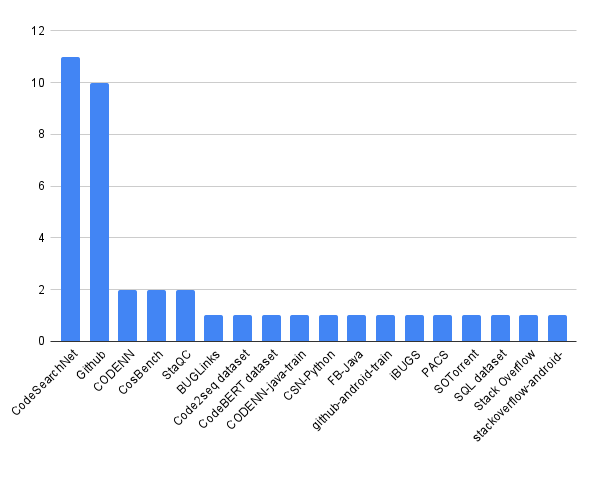
\includegraphics[scale=0.5]{./resources/images/relacionados/datasets.png}
    \smallcaption{Fonte: Autor}
    \label{fig:related-datasets}
\end{figure}

O gráfico \ref{fig:related-metrics} mostra as métricas utilizadas nos estudos em questão. Nota-se que \gls{mrr} e \textit{SuccessRate@k} foram as métricas mais utilizadas para o problema de busca de código.
\begin{figure}[htbp]
    \centering
        \caption{Métricas utilizadas}
        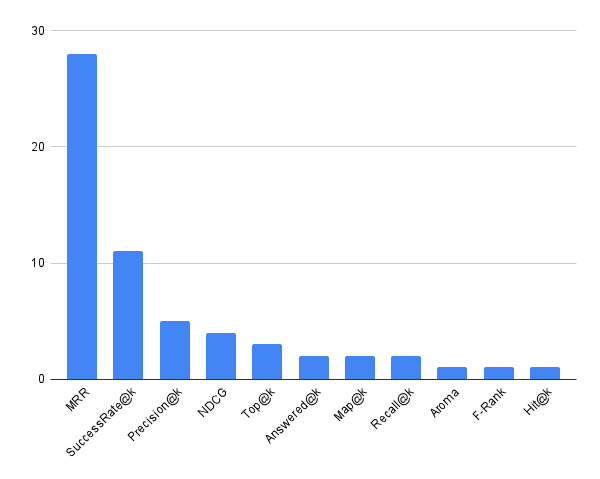
\includegraphics[scale=0.5]{./resources/images/relacionados/metrics.png}
        \smallcaption{Fonte: Autor}
        \label{fig:related-metrics}
\end{figure}

A figura \ref{fig:related-baselines} mostra os modelos de busca de código utilizados como base de comparação nos estudos em questão. Nota-se que a maioria dos modelos utilizam redes neurais profundas, com exceção do \gls{unif}, \textit{Apache Lucene} e \textit{ElasticSearch}. Além disso, nota-se o uso extensivo de modelos \textit{transformers} baseados em \gls{bert}, como \textit{CodeBERT}, \textit{RoBERTa} e \textit{GraphCodeBERT}. Uma possível explicação para o uso de modelos \textit{transformers} é a eficiência de tais modelos quando comparados com outras técnicas como busca textual ou redes neurais profundas.
\begin{figure}[htbp]
    \centering
        \caption{Modelos de comparação utilizados}
        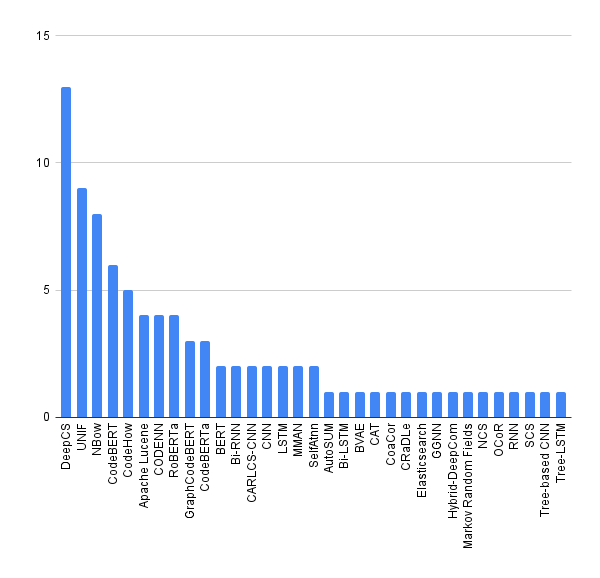
\includegraphics[scale=0.5]{./resources/images/relacionados/baselines.png}
        \smallcaption{Fonte: Autor}
        \label{fig:related-baselines}
\end{figure}

Por fim, a fim de determinar qual o melhor modelo apresentado, concluímos que não é possível realizar tal comparação utilizando os resultados apresentados em seus respectivos estudos. Isso porque, apesar dos experimentos utilizarem as mesmas métricas de busca, os resultados dependem de fatores específicos dos estudos em questão, como a base de dados utilizada.

\chapter{Conceitos}
\label{chp:concepts}
Nesse capítulo serão apresentados os principais conceitos que serão utilizados ao longo da metodologia apresentada.

\section{Sistemas de Busca de Código-Fonte}
Na literatura, encontra-se diferentes técnicas para busca de código-fonte. Porém, antes apresentar uma visão geral do estado da arte, serão definidos alguns termos comumente utilizados nessa área de busca de código-fonte. \textit{Query} é a entrada do sistema - os termos introduzidos pelo usuário para realizar uma busca. A intenção do usuário é o que este quer buscar, e que será expressa através da \textit{query}. Sistemas de busca de código-fonte, por sua vez, consistem em encontrar trechos de código-fonte relevantes à \textit{query} inserida pelo usuário.

Dito isso, \textcite{Grazia2022CodeSA} realizaram uma extensa revisão nos trabalhos da área e, segundo os autores, três fatores são considerados ao desenvolver sistemas de busca de código-fonte. São estes \cite{Grazia2022CodeSA}:
\begin{itemize}
  \item Facilidade de uso: o usuário deve ser capaz de criar \textit{queries} sem treinamento ou conhecimento prévio do sistema.
  \item Expressividade: dada quaisquer intenção do usuário, este deve ser capaz de expressá-la através de \textit{queries}.
  \item Precisão: as \textit{queries} devem ser capazes de expressar a intenção do usuário com o mínimo de ambiguidade.
\end{itemize}

\textit{Queries}, como dito anteriormente, são a interface do usuário com o sistema. Em busca de código-fonte, há diferentes formas de \textit{queries}, dependendo do sistema. 
Trabalhos como \cite{NGUYEN2017CombiningWW}, \cite{Chen2018ANF} e \cite{Du2021IsAS} utilizam \textit{queries} em linguagem natural, como 'busca binária' ou 'binarySearch'. Este formato de \textit{queries} proporciona facilidade de uso e expressividade, enquanto perde em precisão da \textit{query} pelo fato de haver ambiguidades inerentes às linguagens naturais. Sistemas como \textit{Google}, \textit{Stack Overflow} e \textit{Github} utilizam esse formato de \textit{query}.

Trabalhos como \textcite{Zhou2018SLAMPARC}, \textcite{Fujiwara2019CodetoCodeSB} e \textcite{Mukherjee2020SearchingAD} utilizam \textit{queries} no formato de código-fonte. Uma possível \textit{query} desses sistemas seria apenas a declaração de uma função em linguagem de programação. Com isso, o sistema seria responsável por procurar trechos de código-fonte que servissem como corpo dessa função. \textit{Queries} neste formato provêm facilidade de uso, mas a precisão e expressividade variam de acordo com a intenção do usuário \cite{Grazia2022CodeSA}. Por fim, tais sistemas são utilizados, principalmente, para sugestões de código-fonte enquanto o usuário escreve o código.

\textcite{Martie2015CodeExchangeSR} e \textcite{Sivaraman2019ActiveIL} propuseram uma linguagem de busca estruturada, similar às linguagens de banco de dados como SQL para busca de código-fonte. Para encontrar códigos-fonte com os trechos \textit{import math} e \textit{def sum(a, b):}, uma possível \textit{query} válida nesses sistemas seria \textit{'import math' AND 'def sum(a,b):'}. Com essa estrutura de \textit{queries}, tais sistemas provem alta precisão e expressividade, em detrimento da facilidade de uso, pelo fato do usuário precisar aprender uma nova linguagem para realizar as buscas.

Por outro lado, trabalhos como \textcite{Reiss2009SemanticsbasedCS} e \textcite{Jiang2018ResearchPS} recebem a entrada e saída esperadas como \textit{queries}, e buscam códigos-fonte que, dada tal entrada produza a saída correspondente. Por exemplo: dada a entrada esperada 'nOmE' e a saída esperada 'nome', o sistema irá buscar códigos-fonte que produzam tal saída, dada tal entrada. Tal formato de \textit{query} provê facilidade de uso, mas são necessárias muitas \textit{queries} para se alcançar expressividade e, principalmente, precisão. Ainda, tais sistemas possuem aplicações em metodologias de desenvolvimento de \textit{software} como \textit{test-driven development}, onde o usuário primeiro escreve os testes para depois implementar a funcionalidade. A ideia é que, dado os testes (que possuem valores de entrada e saída definidos), o sistema de busca de código-fonte encontre quais trechos de código satisfazem tais testes.

Além disso, há diferentes técnicas de busca de código-fonte na literatura. Trabalhos como \textcite{Lu2015QueryEV} e \textcite{Li2016RelationshipawareCS}, por exemplo, utilizam uma técnica chamada \textit{query expansion}. Nela, dada uma \textit{query} o sistema realiza mais de uma busca com termos similares aos da \textit{query}, a fim de melhorar os resultados da busca. 

Depois, trabalhos como \textcite{Mitra2018AnIT}, \textcite{Gu2018DeepCS} e \textcite{Sun2022CodeSB} utilizam técnicas de \textit{machine learning} no problema de busca de código-fonte a partir de linguagem natural. Durante o aprendizado, estes modelos geram \textit{embeddings} para dois domínios: de linguagem natural e de código-fonte. O primeiro, geralmente são extraídos textos de comentários e documentações, os quais descrevem as tarefas realizadas por determinado código-fonte. O segundo corresponde ao código-fonte em si. Com isso, a similaridade entre a \textit{query} e o código-fonte se dá no espaço vetorial dos \textit{embeddings}.

De forma semelhante, trabalhos recentes como \textcite{Feng2020CodeBERTAP} e \textcite{Guo2021GraphCodeBERTPC} utilizam modelos \textit{transformers} para aprender as relações semânticas entre linguagem natural (da \textit{query} e das descrições dos códigos-fontes presentes nas bases de treinamento) e do código-fonte. Atualmente, tais sistemas são o estado da arte na área de busca de código-fonte.

\section{Aprendizagem de máquina em Processamento de Linguagem Natural}

A aplicação de técnicas de aprendizagem de máquina tem melhorado significativamente o estado da arte da área de processamento de linguagem natural, conforme visto em modelos como \gls{nbow}, \gls{deepcs} e \gls{bert}.

Porém, modelos de aprendizagem de máquina trabalham com números ao invés de texto. Com isso, para utilizar esses modelos dentro da área de \gls{nlp}, utiliza-se um conjunto de técnicas chamado \textit{word embedding}. Tais técnicas criam representações vetoriais a partir de \textit{tokens}, os quais podem então servir como entrada para modelos de aprendizagem de máquina. Desse conjunto de técnicas, destaca-se a família de algoritmos \textit{Word2Vec} \cite{Mikolov2013EfficientEO} \cite{Mikolov2013DistributedRO}.

Os \textit{tokens} utilizados pelo \textit{word embedding} são gerados por algoritmos chamados tokenizadores. Estes algoritmos geram \textit{tokens} a partir de determinado corpus ou bases textuais \cite{Mielke2021BetweenWA}. \textit{Tokens} são unidades menores dos textos, como por exemplo palavras, morfemas ou símbolos específicos do \textit{tokenizador} - portanto, os \textit{tokens} gerados dependem do tokenizador. Em modelos \textit{transformers}, os tokenizadores mais utilizados são \gls{bpe} e \textit{WordPiece}.

O \gls{bpe} inicialmente cria uma lista com todas as palavras distintas do corpus de treinamento. A partir dessa lista, um vocabulário é gerado com todas as letras distintas - e textos com palavras que não estavam no corpus de treinamento serão substituídos pelo token \textit{unknown} (desconhecido). Aqui, vale frisar que modelos transformers como GPT-2 e RoBERTa utilizam uma variação do \gls{bpe} chamada \textit{byte-level} \gls{bpe}, a qual utiliza \textit{bytes} ao invés das letras em formato Unicode, eliminando assim a necessidade do \textit{token} '\textit{unknown}'.

A partir do vocabulário inicial, o \gls{bpe} itera sobre todo o corpus de treinamento para determinar a frequência com que os \textit{tokens} de seu vocabulário ocorrem. Então, são gerados pares (daí o nome \textit{byte-pair}) contendo o \textit{token} e sua frequência no corpus de treinamento. Ao fim, o \gls{bpe} concatena os dois \textit{tokens} dos pares mais frequentes nessa iteração, a fim de criar um novo \textit{token} em seu vocabulário. Tais relações entre \textit{tokens}, aprendidas a partir de suas frequências no corpus de treinamento, são chamadas de regras de \textit{merge}. Por fim, vale notar que, a cada iteração, é adicionado um novo \textit{token} ao vocabulário do tokenizador. E a a quantidade de iterações que o tokenizador fará, e portanto o tamanho de seu vocabulário, é determinada pelo usuário.

O \textit{WordPiece} segue praticamente os mesmos passos do \gls{bpe}, com algumas diferenças da implementação. Inicialmente, o \textit{WordPiece} também gera um vocabulário a partir das palavras distintas que ocorrem no corpus de treinamento. A diferença em relação ao \gls{bpe} é que o \textit{WordPiece} adiciona um prefixo que indica a continuação de determinada palavra, às letras do vocabulário. Por exemplo, dada a palavra $frase$, os seguintes \textit{tokens} serão gerados: $[f, \#\#r, \#\#a, \#\#s, \#\#e]$. Outra diferença em relação ao \gls{bpe} é que, ao invés da frequência, os \textit{tokens} são combinados utilizando uma nota dada pelo \textit{WordPiece} a cada \textit{token}. Essa nota é computada utilizando a seguinte equação:
\begin{equation*}
y=\frac{f_{1,2}}{f_1 \times f_2}
\end{equation*}
onde $y$ é a nota do \textit{token}, $f_{1,2}$ é a frequência do par de \textit{tokens}, $f_1$ a frequência do o primeiro \textit{token} do par e $f_2$ do segundo \textit{token}. Com isso, são gerados os \textit{tokens} de determinado corpus.

Por fim, todos os modelos \textit{transformers} utilizados no capítulo \ref{chp:experiments} utilizam tokenizadores baseados no \textit{WordPiece}. A única excessão é o \gls{bert} \textcite{Devlin2019BERTPO}, que utiliza um tokenizador baseado em \textit{WordPiece}.

\section{Modelos de Atenção}
Modelos \textit{transformers}, como \textit{BERT} e \textit{GPT}, utilizam algum tipo de modelo de atenção (ou mecanismo de atenção). Segundo \textcite{Vaswani2017AttentionIA}, atenção pode ser descrita como uma função de mapeamento entre um vetor \textit{query} $Q$ e um par chave-valor de vetores $K$ e $V$, respectivamente. \textcite{Vaswani2017AttentionIA} propõe uma função de atenção, chamada \textit{Scaled Dot-Product Attention}, a qual é descrita da seguinte forma \cite{Vaswani2017AttentionIA}:
\begin{equation*}
A(Q, K, V)= softmax(\frac{QK^T}{\sqrt{d_k}}) \times V
\end{equation*}
onde $d_k$ é a dimensão do vetor $K$. Como o resultado do $softmax$ consiste em uma distribuição de probabilidades, a multiplicação vetorial do vetor resultante de $softmax(\frac{QK^T}{\sqrt{d_k}})$ com o vetor $V$ ativará alguma dimensão de $V$, indicando assim a atenção de $Q$ e $K$ em $V$, ou $A(Q, K, V)$.

Além disso, os modelos \textit{transformers} utilizam uma técnica chamada \textit{multi-head attention}. Nela, são realizadas projeções lineares dos vetores $Q$, $K$ e $V$, as quais foram aprendidas durante a fase de treinamento \cite{Vaswani2017AttentionIA}. Isso permite com que o modelo consiga observar, de forma conjunta, diferentes representações de determinado \textit{token} em diferentes posições do texto.

A arquitetura \textit{transformer} também prevê um vetor de posição para cada \textit{token}, para descrever sua posição no texto. Esse vetor é chamado \textit{positional encoding} e foi descrito por \textcite{Vaswani2017AttentionIA} da seguinte forma:
\begin{eqnarray*}
PE_{(pos, 2_i)} & = &\sin{\frac{pos}{10000^\frac{2_i}{d_m}}} \\
PE_{(pos, 2_(i+1))} & = & \cos{\frac{pos}{10000^\frac{2_i}{d_m}}}
\end{eqnarray*}
onde $pos$ é a posição do \textit{token}, $d_m$ é a dimensão do modelo e $i$ é a dimensão atual, onde $0 \leq i \leq d$. Como as funções de seno e cosseno são periódicas, os valores gerados estarão entre $2\pi$ e $10000 \times 2\pi$. Com isso, o \textit{positional encoding} é capaz de descrever as posições absolutas e relativas de determinado \textit{token} no texto. Vale frisar que é possível descrever posições relativas neste modelo pois, dado um intervalo $k$ entre um \textit{token} e outro \textit{token} anterior, $PE_{pos+k}$ pode ser representado como função linear de $PE_{pos}$ \cite{Vaswani2017AttentionIA}.

Por fim, a figura \ref{fig:transformer-architecture} mostra um diagrama com uma visão geral da arquitetura \textit{transformer}:

\begin{figure}[H]
    \centering
    \caption{Visão geral da arquitetura \textit{Transformer}}
    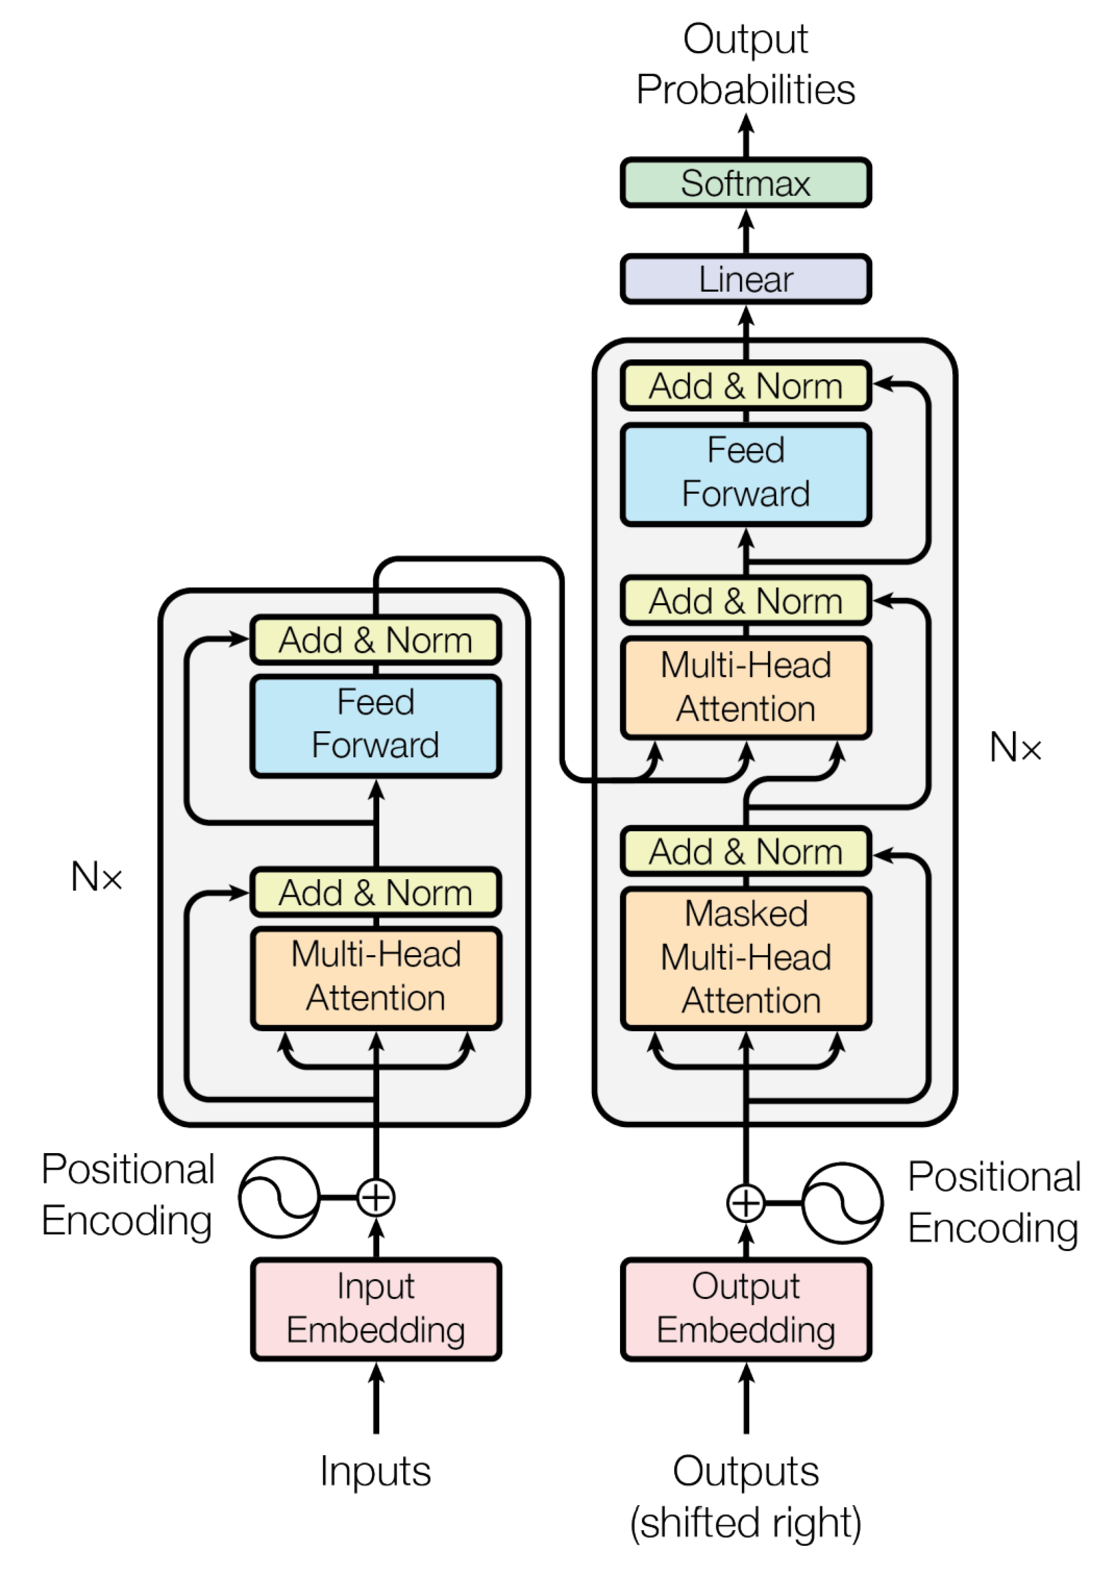
\includegraphics[scale=0.4]{resources/images/conceitos/transformer-architecture.pdf}
    \smallcaption{Fonte: \cite{Vaswani2017AttentionIA}}
    \label{fig:transformer-architecture}
\end{figure}

Vale frisar que o \textit{pipeline} do lado esquerdo da figura, o qual recebe os \textit{embeddings} de entrada (\textit{input embeddings)}, é chamado de \textit{encoder}. E o \textit{pipeline} do lado direto, que recebe os \textit{embeddings} de saída (\textit{output embeddings}) e o resultado do \textit{encoder}, é chamado de \textit{decoder}.

A arquitetura da figura \ref{fig:transformer-architecture} foi aplicada inicialmente ao modelo \gls{gpt}, e atingiu o estado da arte em tarefas de tradução \cite{Vaswani2017AttentionIA}.

Posteriormente, foi proposto o modelo \gls{bert} \cite{Devlin2019BERTPO}. A principal diferença para o \gls{gpt} é a capacidade de aprender, dado um \textit{token} do texto, o contexto tanto com os \textit{tokens} anteriores quanto com seus sucessores. Em outras palavras, o \gls{bert} aprende o contexto de forma bi-direcional.

Os outros modelos citados no capítulo \ref{chp:experiments} são derivados do \gls{bert} ou do \gls{gpt}. O \gls{roberta} melhorou a fase de pré treino do \gls{bert} através de ajustes de seus hiperparâmetros \cite{Liu2019RoBERTaAR}. O \gls{codebert} busca otimizar o \gls{bert} para tarefas que envolvam processamento de código-fonte, adicionando o par código-fonte/comentário em linguagem natural ao modelo \textit{transformer} \cite{Feng2020CodeBERTAP}. O \gls{graphcodebert} também busca otimizar tarefas que envolvam textos de código-fonte, porém utiliza uma estrutura chamada \textit{data flow} para extrair informações do código-fonte \cite{Guo2021GraphCodeBERTPC}. Por fim, o \gls{gpt2} adicionou novos hiperparâmetros e novos dados à sua base de treinamento, em relação ao seu antecessor \gls{gpt} \cite{Radford2019LanguageMA}.

\section{Métricas de Avaliação de Recuperação de Informação}
Dado uma lista de resultados para determinada busca, ordenados de maneira decrescente de relevância, o \gls{mrr} é um valor, entre 0 e 1, que representa em qual posição o resultado mais relevante estará na lista de resultados. Caso o \gls{mrr} seja 1, o resultado mais relevante estará (na maioria dos casos) em primeiro lugar na lista de resultados; se for 0.5, este estará na segunda posição e assim por diante \cite{Craswell2009}. Vale frisar que essa métrica é composta pela a média entre os resultados de várias buscas em determinada base de dados. Os valores individuais de cada busca são chamados de \gls{rr} e são calculados da seguinte forma:
\begin{equation*}
    RR_i=1/rank_i
\end{equation*}
onde $rank_i$ é a posição de determinado resultado - se este estiver na primeiro posição, $RR=1/1=1$; se estiver na segunda, $RR=1/2=0.5$ e assim por diante. Com isso, tem-se que o \gls{mrr} é a média harmônica de todos os \glspl{rr} para a quantidade de buscas realizadas em determinada base de dados. Daí, tem-se a fórmula do \gls{mrr}:
\begin{equation*}
    MRR = \frac{1}{|Q|} \times \sum_{i=1}^{|Q|} RR_i
\end{equation*}
onde $|Q|$ é a quantidade de buscas realizadas.

Por sua vez, \textit{SuccessRate@k} é um valor, entre 0 e 1, que representa a porcentagem de resultados corretos que estão nas primeiras $k$ posições da lista de resultados. Essa métrica é descrita pela fórmula \cite{Wan2019MultimodalAN}:
\begin{equation*}
    SuccessRate@k=\frac{1}{|Q|} \times \sum_{i=1}^{|Q|} \delta(FRank_i \geq k)
\end{equation*}
onde $\delta(x)$ é uma função que retorna 1 caso x for verdadeiro e 0 caso contrário. $FRank_i$ é a posição do primeiro resultado relevante na lista de resultados \cite{Raghothaman2016SWIMSW}.


\chapter{METODOLOGIA}
\label{chp:methodology}
\graphicspath{ {./resources/images/metodologia} }

O objetivo do presente estudo é comparar modelos de \textit{embeddings} para recuperação de código-fonte a partir de buscas feitas em linguagem natural. Para tanto, propõe-se um sistema para a comparação de \textit{embeddings} gerados por \textit{encoders} tanto de linguagem natural quanto de código-fonte.
O presente estudo propõe um sistema, apresentado na figura \ref{fig:metodology-system_overview}, que servirá para comparar modelos de \textit{embeddings} para recuperação de código-fonte a partir de buscas feitas em linguagem natural.

\begin{figure}[htbp]
    \centering
        \caption{Visão geral do sistema}
        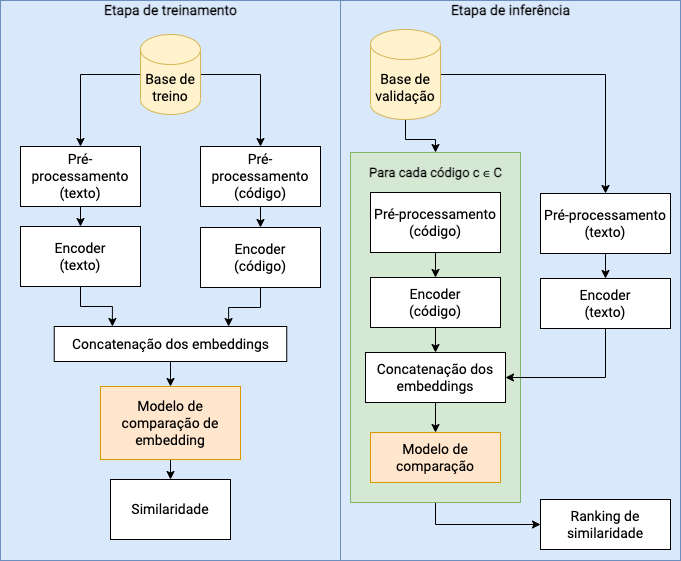
\includegraphics[scale=0.5]{system-overview.png}
        \smallcaption{Fonte: Autor}
        \label{fig:metodology-system_overview}
\end{figure}

\section{Base de Dados}
Todos os experimentos serão realizados utilizando os dados disponibilizados na pela \textit{Microsoft} através do repositório \textit{CodeSearchNet} \cite{Husain2019CodeSearchNetCE}. Esse repositório consiste em uma coleção de bases de dados e métricas voltadas ao problema de busca de código usando linguagem natural.

Para os experimentos do estudo em questão, será utilizada a base de dados principal dessa coleção. Tal base contém dois milhões de pares código-fonte/comentário, vindos de bibliotecas de código aberto. Desses pares existentes na base, os comentários são textos, escritos em inglês, que descrevem o código-fonte correspondente. O código-fonte, por sua vez, são trechos de código-fonte que realizam determinada tarefa. Além disso, nessa base pode-se encontrar pares com código-fonte das linguagens de programação \textit{Python}, \textit{Javascript}, \textit{Ruby}, \textit{Go}, \textit{Java} e \textit{PHP}. Neste trabalho, serão selecionados os pares código-fonte/comentário das linguagens \textit{Java} e \textit{Python}. Essas duas linguagens foram escolhidas por suas diferenças no sistema de tipagem: a primeira é fortemente tipada, enquanto a segunda é fracamente tipada. 

\section{Pré-processamento}
\label{sec:methodology:pre-processing}
Para cada par código-fonte/descrição, serão feitos dois pré-processamentos em paralelo: um para o código-fonte e um para a descrição. Ambos os pré-processamentos serão realizados a fim de normalizar tais dados para servirem de entrada aos \textit{encoders}, detalhados na seção \ref{sec:methodology:encoders}. Tanto para o código-fonte quanto para a descrição serão utilizados tokenizadores específicos para cada \textit{encoder} selecionado para os experimentos, conforme visto na figura \ref{fig:metodology-tokenizers}.

\begin{figure}[htbp]
    \centering
        \caption{Tokenizadores e \textit{encoders}}
        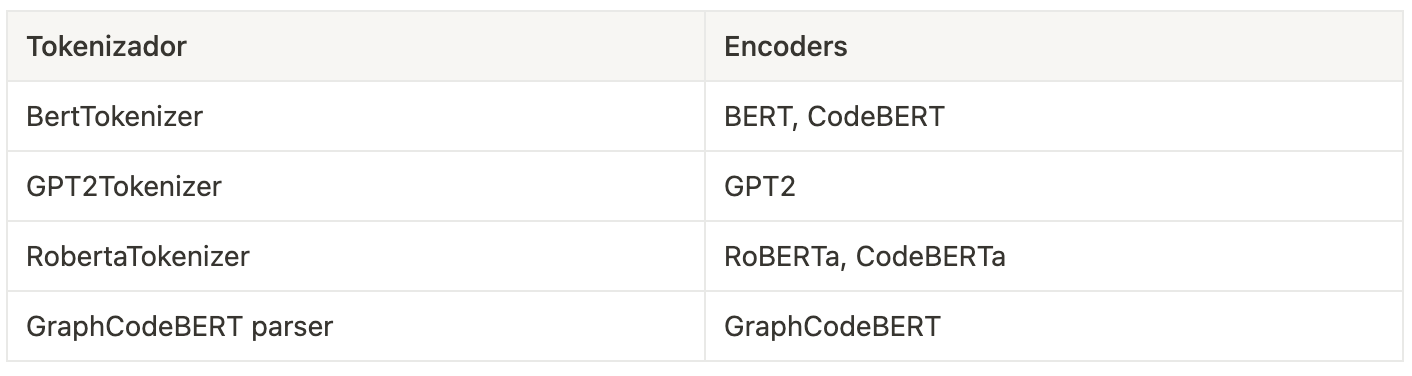
\includegraphics[scale=0.5]{tokenizers.png}
        \smallcaption{Fonte: Autor}
        \label{fig:metodology-tokenizers}
\end{figure}

\section{\textit{Encoders}}
\label{sec:methodology:encoders}
Os \textit{encoders}, relacionados na figura \ref{fig:metodology-tokenizers}, receberão os dados pré-processados para gerar os \textit{embeddings} correspondentes. Com isso, a partir dos pares código-fonte/descrição, essa etapa irá gerar pares de \textit{embeddings} código-fonte/descrição.

\section{Concatenação dos \textit{embeddings}} 
\label{sec:methodology:embeddings-concat}
Com os pares de \textit{embeddings} código-fonte/descrição gerados, esta etapa será responsável por concatenar os \textit{embeddings} contidos nesses pares. 
A concatenação desses dois \textit{embeddings} se dará juntando os dois vetores em um só, de forma que dado o primeiro vetor tenha tamanho $m$ e o segundo $n$, o tamanho do vetor resultante após a concatenação será $m + n$.
O \textit{embedding} concatenado resultante servirá como entrada para o modelo de comparação de \textit{embeddings}, descrito a seguir.

\section{Modelo de comparação de \textit{embeddings}}
\label{sec:methodology:embedding-comparator}
O modelo de comparação de \textit{embeddings} consiste em uma rede neural que, a partir de dois \textit{embeddings} concatenados, tem como objetivo determinar a similaridade entre estes dois \textit{embeddings}. A figura \ref{fig:metodology-embeddings_comparator} mostra o diagrama do modelo em questão.

\begin{figure}[htbp]
    \centering
        \caption{Comparador de \textit{embeddings}}
        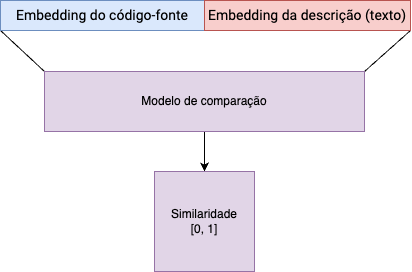
\includegraphics[scale=0.6]{emb-comparator.png}
        \smallcaption{Fonte: Autor}
        \label{fig:metodology-embeddings_comparator}
\end{figure}

Conforme apresentado no diagrama, o comparador consiste em uma rede neural, com $n$ camadas e uma função de ativação. Essa rede receberá como entrada os \textit{embeddings} do código-fonte e de sua descrição, concatenados. A saída será um valor, entre 0 e 1, que representará a similaridade entre os dois \textit{embeddings} da entrada. Tanto a topologia, quanto o número de camadas e a função de ativação serão determinados experimentalmente, conforme descrito no capítulo \ref{chp:experiments}.

\section{Etapa de inferência}
Por fim, após a etapa de treinamento do modelo de comparação de \textit{embeddings}, será realizada a etapa de inferência. Conforme descrito na figura \ref{fig:metodology-system_overview}, cada texto da base de validação será comparado com todos os códigos-fonte da mesma base, a fim de gerar um \textit{ranking} de similaridade dos códigos-fonte com o texto em questão. Esse texto representa uma consulta feita pelo usuário, em linguagem natural, ao procurar por determinado código-fonte.
Essa etapa de inferência servirá para validar o modelo de comparação. Os resultados obtidos a partir dessa etapa serão estudados de acordo com o capítulo \ref{chp:experiments}.



\label{chp:experiments}
\chapter{PROPOSTA EXPERIMENTAL}

Para o estudo em questão, propõe-se três experimentos. Os objetivos e a descrição detalhada de cada um destes experimentos estão nas seções a seguir.


\section{Definição do modelo do comparador}
\label{sec:experiments:emb-comparator}
O objetivo desse experimento é definir os parâmetros do comparador de \textit{embeddings}. Os parâmetros utilizados, bem como os valores para cada um neste experimento, se encontram na lista abaixo.

\begin{itemize}
    \item topologias: \gls{resnet} e \gls{mlp}
    \item número de camadas escondidas: 2, 4, 6 e 8
    \item função de ativação: \gls{tanh} e \gls{relu}
    \item \textit{dropout}: 5, 10, 15 e 20
    \item regularização L1 e L2: 0.001, 0.01 e 0.1
\end{itemize}

Vale frisar que tais valores foram escolhidos de forma empírica, durante a concepção desse experimento. 

Além disso, para variar os valores no modelo de comparação, é necessário que os \textit{encoders} de código-fonte e texto estejam fixos. Com isso, para este experimento, foi escolhido, de forma empírica, o par de \textit{encoders} código-fonte/texto \textit{CodeBERT} e \textit{BERT}.

\section{Comparação entre \textit{encoders}}
\label{sec:experiments:encoders}
Com os parâmetros do comparador de \textit{embeddings} definidos pelo experimento \ref{sec:experiments:emb-comparator}, este experimento será realizado para comparar pares de \textit{embeddings} de diferentes \textit{encoders}. Para tanto, foram escolhidos seis \textit{encoders}, conforme mostra a \ref{fig:experiments-encoders}.

\begin{figure}[htbp]
    \centering
        \caption{\textit{Encoders} selecionados}
        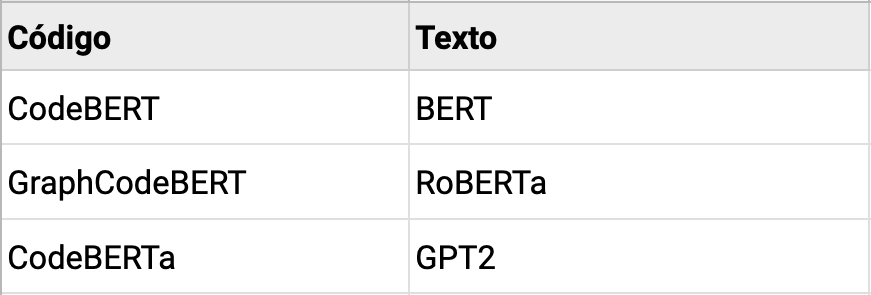
\includegraphics[scale=0.5]{resources/images/metodologia/encoders-list.png}
        \smallcaption{Fonte: Autor.}
        \label{fig:experiments-encoders}
\end{figure}

Com isso, 8 pares de \textit{encoders} serão utilizados nesse experimento; isso porque um par de \textit{encoder} já foi utilizado no primeiro experimento, eliminando, portanto, a necessidade de utilizá-lo novamente. A ideia central desse experimento é analisar como que o modelo de comparação se comporta com diferentes topologias de \textit{encoders}, e seus respectivos \textit{embeddings}.

\section{Generalização dos \textit{encoders}}
\label{sec:experiments:generic_encoder}
Por fim, o objetivo desse experimento é avaliar se o modelo de comparação é capaz de abstrair os \textit{encoders} utilizados no sistema.

Para tanto, será criada uma base de pares de \textit{embeddings} código-fonte/texto. Tais \textit{embeddings} serão gerados a partir de todos os nove pares possíveis formados pelos \textit{encoders} da figura \ref{fig:experiments-encoders}. Então, será realizado apenas um treinamento com todos os pares de \textit{embeddings} da base.

Com isso, a hipótese desse experimento é que se o modelo de comparação obtiver bons resultados nesse cenário, então este é capaz de abstrair os \textit{encoders} utilizados para geração dos \textit{embeddings}. Em outras palavras, dado quaisquer pares de \textit{encoders} (formados pelos \textit{encoders} da figura \ref{fig:experiments-encoders}) código-fonte/descrição, o modelo de comparação será capaz de determinar a similaridade dos \textit{embeddings} gerados.

\chapter{Cronograma}

A figura \ref{fig:introduction:agenda} mostra um cronograma para as atividades previstas para o estudo em questão.

\begin{figure}[H]
    \centering
    \caption{Cronograma}
    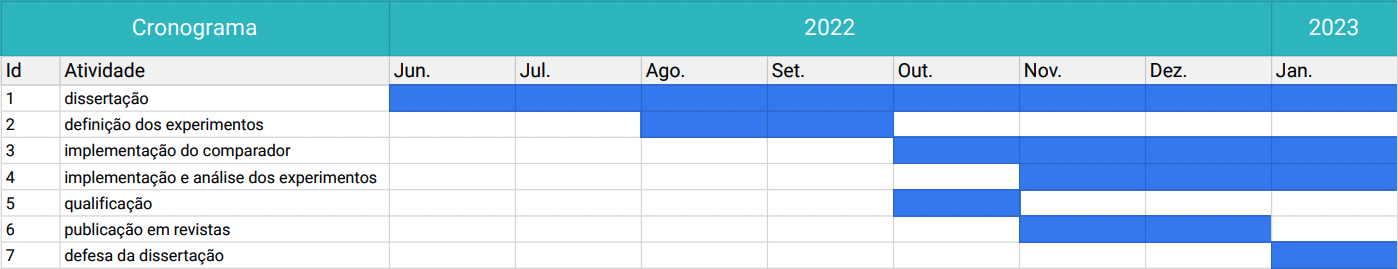
\includegraphics[width=1.0\textwidth]{resources/images/introducao/agenda.png}
    \smallcaption{Fonte: o Autor}
    \label{fig:introduction:agenda}
\end{figure}



\printbibliography

% \appendix
% \chapter{METODOLOGIA DA REVISÃO SISTEMÁTICA \label{appendix:revisao-literatura}}

Uma busca sistemática da literatura foi realizada e os seguintes parâmetros se destacam:
\begin{itemize}
   \item \textbf{Query de busca}:  \enquote{cid E aprendizado E maquina}, \enquote{codigo E icd}, \enquote{ehr E classification}, \enquote{ehr E ensemble E learning E word2vec E fasttext}, \enquote{ehr E mimic E embedding E similarity}, \enquote{ehr E word2vec}, \enquote{icd E bert}, \enquote{icd E classification}, \enquote{icd E deep E learning}, \enquote{mimic E ensemble E learning}, \enquote{mimic E lstm}, \enquote{mimic E rnn}, \enquote{mimic E transformer}, \enquote{mimic-III E word2vec E similarity}, e \enquote{subwording E tokenization};
   \item \textbf{Motor de busca}: \textit{google.com.br}, \textit{scholar.google.com.br}, e \textit{semanticscholar.org};
   \item \textbf{Variável de exclusão}: ano de publicação menor que 2016.
\end{itemize}
 
 Para cada documento encontrado, a seguinte tabela foi preenchida:
 \begin{itemize}
   \item Título do artigo;
   \item Data da publicação;
   \item O objetivo principal do documento;
 \end{itemize}
 
 Quando o objetivo principal do documento encontrado se relacionava com o objetivo principal desse trabalho, os seguintes campos eram preenchidos:
 \begin{itemize}
   \item A necessidade da pesquisa;
   \item A metodologia apresentada;
   \item O resultado final e trabalhos futuros;
  \end{itemize}
  
Ao final dessa etapa, 66 documentos constavam na tabela. Após uma análise das informações, 29 documentos foram selecionados como relevantes. Um estudo detalhado desses documentos foi realizado e o processo de \textit{snowballing} foi empregado para identificar documentos adicionais relevantes para compor as referências.

Além disso, referências usualmente utilizadas na área de \gls{pln}, notoriamente as quais possuem um elevado número de citações, não passaram pelo processo descrito anteriormente.

\end{document}